
%What is eels?
%Sample experimental setup
%Sample spectra
%Signal types
%usages
%pros, cons/ STEM TEM
\setcitestyle{numbers,open={[},close={]}}
Having described the inner workings of EELS and DFT, we will now investigate how we can use the ground state density and the Kohn-sham wavefunctions and eigenvalues to calculate the features of an EELS spectra.  Central to this challenge, is the fact that DFT is however a ground state theory; the Hohenberg Kohn theorems only guarantee that agreement between the calculation and reality for the lowest energy state \cite{hohenberg_inhomogeneous_1964}. As EELS inherently involves exciting an atom above this ground state, a number of assumptions must be made to address this issue. The various approaches to the issue of handling excitations are defining features of many of the techniques used to calculate EELS.  Additionally, the varying requirements of the wide array of features in EELS spectra further diversify the techniques. Broadly, there are three methods for calculating EELS: multiple scattering, atomic multiplet and band structure methods.  We will focus on a number of the band structure methods as well as their advantages and applicability below.


\subsection{Time Dependent Density Functional Theory -TDDFT}
In TDDFT, the EELS spectrum is computed through the macroscopic dielectric function ($\epsilon_{\mathrm{M}}$). As is the case with many EELS calculations, we begin from Fermi's Golden Rule, and define matrix elements which determine the probability of an electron being driven to a new state by some propagator:

\begin{equation}
M_{nm\textbf{k}} = \mel{n\textbf{k}}{e^{-i(\textbf{q+G})\textbf{r}}}{n'\textbf{k+q}}
\label{FGR}
\end{equation}

Where $\textbf{q}$ is the momentum transfer from the beam to the sample and \textbf{G} is the Fourier coefficient of the probe. The initial and final states are the key parameters taken from DFT \cite{exciting}.  These matrix elements can be used to determine the independent particle polarizability $\chi^{\mathrm{KS}}$ \cite{exciting}: 


\begin{equation}
\chi^{\mathrm{KS}}_{\mathrm{\textbf{G,G'}}}(\textbf{q},\omega)=\frac{1}{V}\sum_{nm\textbf{k}}\frac{f_{n\textbf{k}}-f_{m\textbf{k+q}}}{\epsilon_{n\textbf{k}}-\epsilon_{m\textbf{k+q}}+\omega + i\delta} M_{nm\textbf{k}}(\textbf{q,G})M^*_{nm\textbf{k}}(\textbf{q, G'})
\end{equation}

Where $f_{n\textbf{k}}$ is the fermi distribution and V is the volume of the cell.  $\chi^{\mathrm{KS}}$ can be related to the reducible polarizability through the Dyson equation:  

\begin{equation}
\chi = \chi_{\mathrm{KS}} + \chi_{\mathrm{KS}}(\nu + f_{\mathrm{xc}})\chi
\end{equation}

Where $f_{\mathrm{xc}}$ is the exchange and correlation potential.  A common approximation is to set this to zero, a method called the Random Phase Approximation (RPA) \cite{optic}.  At this point we also make two more approximations.  We first assume that $\textbf{q} \to 0$, referred to as the optical limit.  This assumes that the momentum transfer to the sample is minimal, an approach that is valid for low energy losses ($<$50 eV).  We also assume that the probe wavelength is much larger than the resulting perturbations, ($\textbf{ G} \to 0$). This is know as ignoring local field effects.  Both of these approximations can be relaxed on a case by case basis, however this comes at increased computational cost \cite{exciting}. With these approximations, we can proceed to calculate first element of the dielectric tensor: 
\begin{equation}
\epsilon_{\mathrm{00}}^{-1} (\textbf{q},\omega) =1+v \chi
\end{equation}

from which we can calculate the macroscopic dielectric function which relates to the energy loss function: 

\begin{gather}
[\epsilon_{\mathrm{M}}(\textbf{q},\omega)]^{-1} = \epsilon_{\mathrm{00}}^{-1}(\textbf{q},\omega)\\
	L(\textbf{q},\omega) = -\mathrm{Im}[\epsilon_{\mathrm{M}}(\textbf{q},\omega)]^{-1}
\end{gather}

The energy loss function is what is directly measured by EELS and is the standard of comparison for TDDFT. TDDFT is accurate for low losses, so ideal for calculations of plasmons, and in the limit of the optical approximation low energy M edges of transition metals and the lithium K edge \cite{mauchamp_local_2008}.  Limitations of the approach are that it is based on the final state rule, and thus is susceptible to excitonic effects in $\bra{f}$.  Additionally, local field effects can require subtle interpretations and come at computational cost to include \cite{mauchamp_local_2008}.    TDDFT is also applicable to x-ray absorption spectroscopy where the optical limit is more valid.  The only required modifications to the theory are a modification to the propagator in Eq. \ref{FGR} \cite{ankudinov_real-space_1998}:
\begin{equation}
e^{i\textbf{q}\cdot\textbf{r}} \to e^{i\textbf{k}\cdot\textbf{r}}\epsilon \cdot \textbf{r}
\label{x-prop}
\end{equation}

\subsection{Cross Section Approach}
TDDFT is a suitable choice for low loss EELS.  For higher energy ionization edges with non-negligible momentum transfer, Fermi's Golden Rule can be used to compute a double differential cross section instead of the dielectric function.  The differentials are with respect to energy and scattering angle, the two relevant parameters in an EELS experiment.  The relationship is given by \cite{hebert_practical_2007}:

\begin{equation}
		\frac{\partial^2 \sigma}{\partial \Omega \partial E} = \left[\frac{4\gamma^2}{a_{\mathrm{0}^2q^4}}\right] \frac{k_f}{k_i} \sum_{i,f}|\mel{f}{e^{i\textbf{q}\cdot\textbf{r}}}{i}|^2\delta(E-E_f+E_i)
		\label{telnes_eq}
\end{equation}

Where $a_0$ is the Bohr radius, $E$ the energy loss and $\gamma = \sqrt{1- \beta^2}$, the relativistic factor.  As in TDDFT, the approach can be modified to solve for XAS, by replacing the Rutherford cross section with the Thompson cross section in the prefactor and changing the propagator according to Eqn. \ref{x-prop}.



The cross section formalism can also be modified to account for anisotropic samples as well as some experimental parameters \cite{hebert_practical_2007}. Similar to TDDFT, the essential parameters are the initial and final states, taken from DFT ($\bra{f}$ and $\ket{i}$).  The simpler approach with fewer approximations can be attributed to the states being investigated: in low loss EELS, both the initial and final states depend heavily on the band structure, whereas for core losses the initial states are relatively constant and well defined \cite{hebert_practical_2007}.  Cross section methods however still suffer from the limitations of a one particle final state rule approach and their lack of ability to deal with excitonic effects.  

\subsection{Beth Salpeter Equations -BSE}

The largest drawback of TDDFT and cross section calculations is the single particle formalism, which prevents proper treatment of excitonic effects. Solving the BSE is a two particle method that rigorously calculates the  interaction between the excited electron and the resulting hole in the core state \cite{salpeter_relativistic_1951}.  It is applicable to both low and core loss EELS calculations \cite{exciting}.  The core of the BSE is in solving the eigenvalue problem involving the effective two particle Hamiltonian \cite{draxl_bse_2009}: 


\begin{equation}
\hat{H}_{\mathrm{eff}} \ket{A_\lambda} = E_\lambda \ket{A_\lambda}
\end{equation}


The effective Hamiltonian can be broken into three parts, the diagonal, exchange and correlation components\cite{draxl_bse_2009}. \\
The diagonal component which accounts for single particle transitions:
\begin{equation}
	H_{v c \textbf{k}, v' c'\textbf{k'}}^{(\mathrm{diag})} = (\epsilon_{c\textbf{k}}-\epsilon_{v \textbf{k}})\delta_{vv'}\delta_{cc'}\delta_{\textbf{kk'}}
\end{equation}

The exchange component which accounts for the repulsive interaction between the excited electron and its hole: 
\begin{equation}
	H_{v c \textbf{k}, v' c'\textbf{k'}}^{(\mathrm{x})} = \int d^3\textbf{r}\int d^3\textbf{r'}\varphi_{v\textbf{k}}(\textbf{r})\varphi_{c\textbf{k}}^*(\textbf{r})\bar{v}(\textbf{r,r'})\varphi_{v'\textbf{k'}}^*(\textbf{r'})\varphi_{c'\textbf{k'}}(\textbf{r'})
\end{equation}

Where $\varphi$ are the single particle states of the hole and electron and $\bar{v}$ is the unscreened Coulomb potential.  Thirdly, there is the correlation component accounting for the attractive interaction between hole and electron:

\begin{equation}
	H_{v c \textbf{k}, v' c'\textbf{k'}}^{(\mathrm{c})} = -\int d^3\textbf{r}\int d^3\textbf{r'}\varphi_{v\textbf{k}}(\textbf{r})\varphi_{c\textbf{k}}^*(\textbf{r})W(\textbf{r,r'})\varphi_{v'\textbf{k'}}^*(\textbf{r'})\varphi_{c'\textbf{k'}}(\textbf{r'})
\end{equation}

Where W is the screened Coulomb potential on the hole. By treating the hole created by the excited electron as a particle, solving the BSE produces vastly superior results to single particle approaches, particularly in those with moderate screening \cite{draxl_bse_2009}.  However, this method is vastly more computationally demanding and can only be performed on the simplest of structures.   This large computational trade off has led to the continued prevalence of single particle techniques.
%two particle technique
%No CH


\subsection{Core Hole Approximation} \label{Core Hole Approximation}
The computational cost of the BSE method and the difficulties in handling excitonic effects in the single particle approaches has resulted in further approximations being made to improve single particle results.  The most significant of these is the core hole approximation.  This approximation is centred on artificially exciting a DFT into an excited one in order to better calculate the final states in EELS, $\bra{f}$.  Early implementations involved replacing the excited atom with the next element on the periodic table, called the Z+1 approach \cite{lee_new_1977}.  This method was mildly successful, however it lacks the flexibility to handle excitations from different shells, and has since been largely replaced with the core hole approximation \cite{hebert_practical_2007}.  The core hole approximation involves manually decreasing the occupancy of an excited state, and adding the additional charge to the background to conserve electron number \cite{wien2k}. The effectiveness of the approximation however has been mixed.  In some cases, including a core hole results in excellent agreement with experiment, whilst in others, ignoring a core hole produces more accurate results.   There have been a number of offered explanations based on the nature of the material: eg. insulators require a hole and metals do not.  These general rules have not been successful in predicting all cases and more involved techniques based on density of states maps have also been proposed \cite{mauchamp_core-hole_2009}.  In general however, spectra tend to fall in between the two extremes, which has led to some \textit{ad hoc} approaches of including non integer core holes, so as to best fit experiment, see Fig \ref{core-hole-types} \cite{hebert_practical_2007, luitz_partial_2001, hebert_improvement_2003, slater_energy_1964}. This state of affairs has remained unchanged for the past 30 years and consistently leads to unsatisfying results \cite{ brydson_further_1988, hardcastle_robust_2017,bad_hole1,bad_hole2, bad_hole3, bad_hole4, bad_hole5, bad_hole6, bad_hole7, bad_hole8,bad_hole9, bad_hole10}. \\
The treatment of core holes is particularly problematic in lithium as core state are very shallow with only a single other core electron to shield it.  The shallow shielded hole means that every lithium compound will exhibit some degree of core hole effects.  Consequently, in order to  calculate lithium ELNES a more rigorous approach to core hole screening is required.  Developing a deterministic method of introducing non-integer core holes for this end is the focus of this work


\begin{figure}
	\begin{subfigure}{0.45\textwidth}
		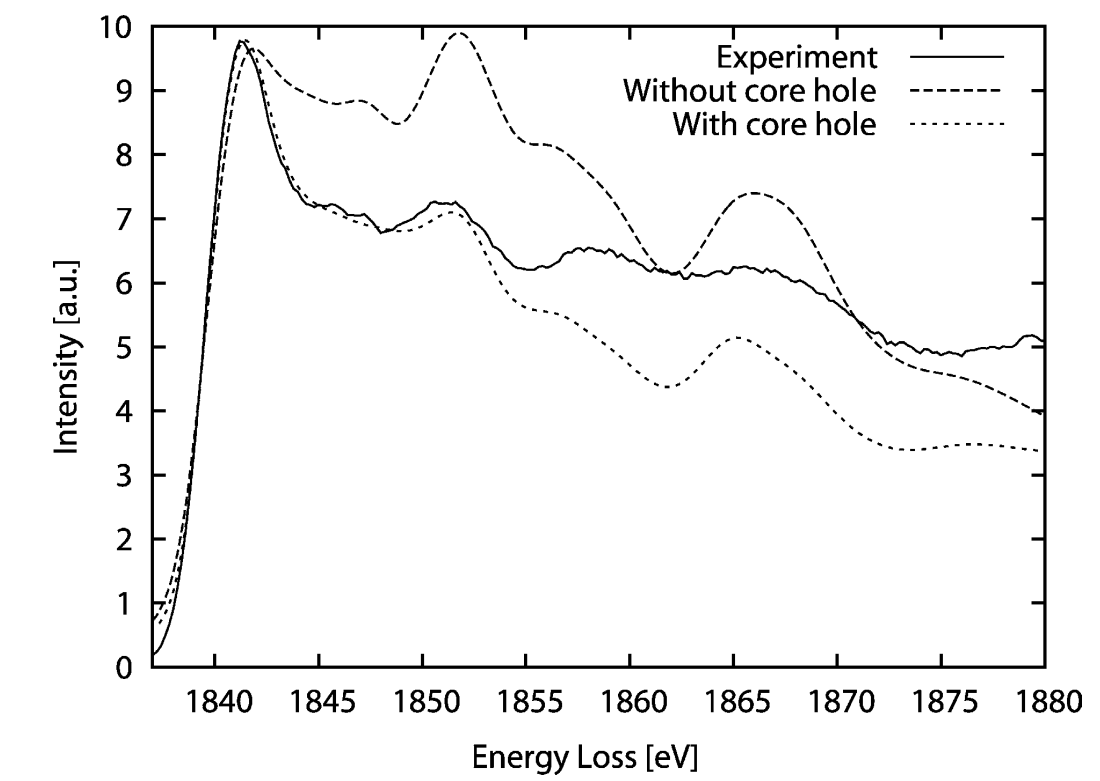
\includegraphics[width=1\textwidth]{hebert_ch_si_good.png} 
		\caption{}
		\label{hebert-ch-good}
	\end{subfigure}
    \hspace{-0.01cm}
	\begin{subfigure}{0.45\textwidth}
		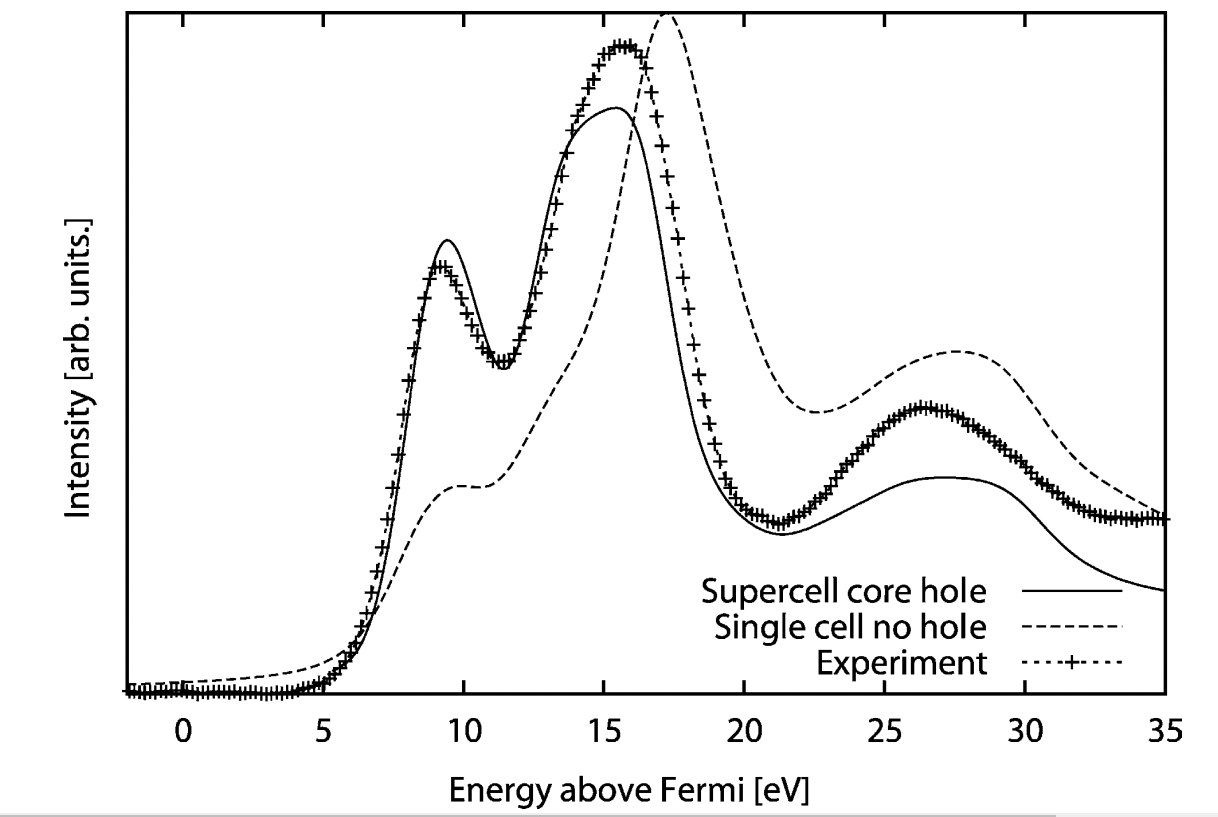
\includegraphics[width=1\textwidth]{hebert_ch_mg} 
		\caption{}
		\label{hebert-ch-bad}
	\end{subfigure}
	\vspace{1cm}
	\begin{subfigure}{0.45\textwidth}
		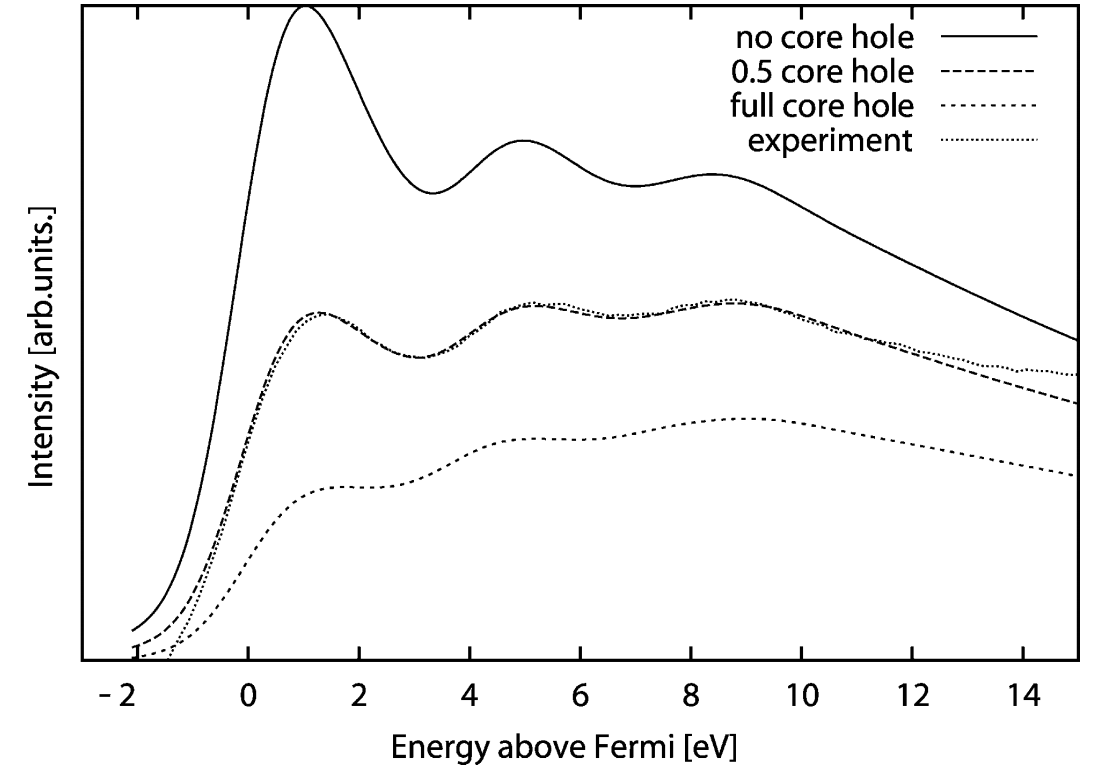
\includegraphics[width=1\textwidth]{luitz_cu_half} 
		\caption{}
		\label{luitz_half}
	\end{subfigure}
	\centering
	\caption{The three typical results of inserting a core hole. In (a) the core hole results in good agreement with experiment.  In (b) and (c), the core hole overestimates the excitonic effects, resulting in errors in peak intensity.  In (c), an \textit{ad hoc} fractional core hole is inserted resulting in good agreement at the cost of physicality. Results from \cite{hebert_improvement_2003} (a,b) and \cite{luitz_partial_2001} (c).}
	\label{core-hole-types}
	
\end{figure}

\newpage




